\documentclass{article}
\usepackage{graphicx}
\begin{document}

\section*{Examples of calculations by Pulsed Laser Polymerization (PLP) plugin with mcPolymer}

\vspace{10mm}

\subsection*{Example 1}


M. Buback, M. Busch, R. A. Lämmel, \textit{Macromol. Theory Simulations} \textbf{1996}, 5, 845.

\begin{figure}[h]
\centering
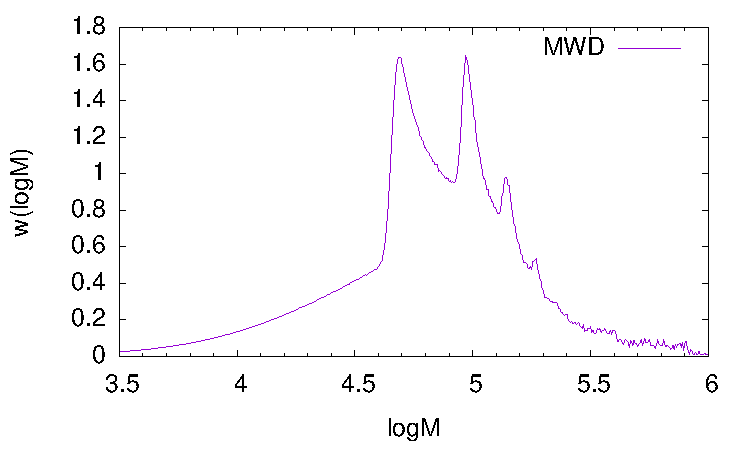
\includegraphics[width=0.77\textwidth]{plp_example1.pdf}
\caption{Results of calculations by mcPolymer with PLP plugin.}
\end{figure}

\begin{figure}[h]
\centering
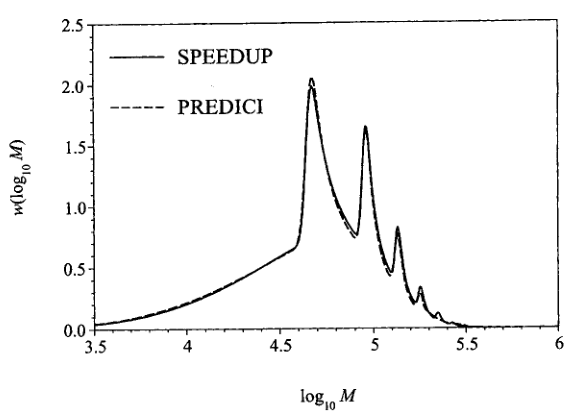
\includegraphics[width=0.77\textwidth]{Buback1996_PLP.png}
\caption{Results of calculations by PREDICI published in the paper.}
\end{figure}

\subsection*{Example 2}

P. Vana, L. H. Yee, C. Barner-Kowollik, J. P. A. Heuts, T. P. Davis, \textit{Macromolecules} \textbf{2002}, 35, 1651.

\begin{figure}[h]
\centering
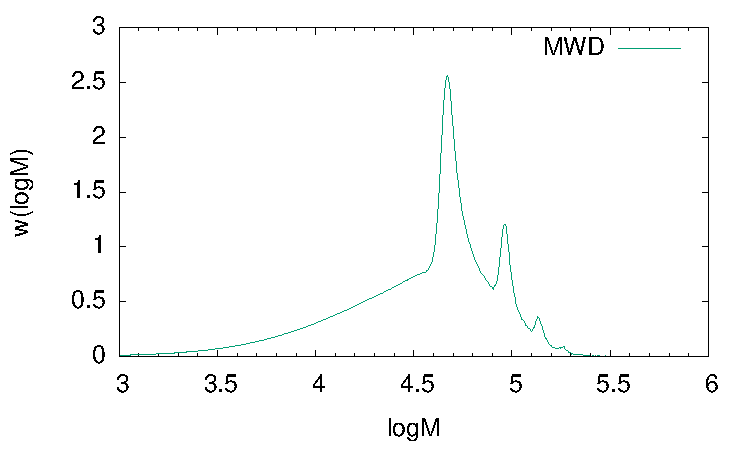
\includegraphics[width=0.77\textwidth]{plp_example2.pdf}
\caption{Results of calculations by mcPolymer with PLP plugin.}
\end{figure}

\begin{figure}[h]
\centering
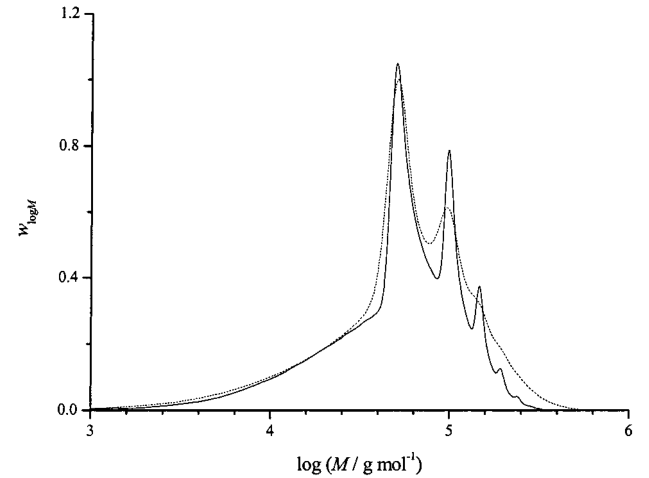
\includegraphics[width=0.77\textwidth]{Vana2002_PLP.png}
\caption{Results of calculations by PREDICI published in the paper.}
\end{figure}

\vspace{5mm}

\subsection*{Example 3}
Wulkow, Michael. "PREDICI—A Software Package for Real-life Polymerisation Kinetics." Progress in Industrial Mathematics at ECMI 94. Vieweg+Teubner Verlag, \textbf{1996}. 166-175. DOI:10.1007/978-3-322-82967-2\_20

\begin{figure}[h]
\centering
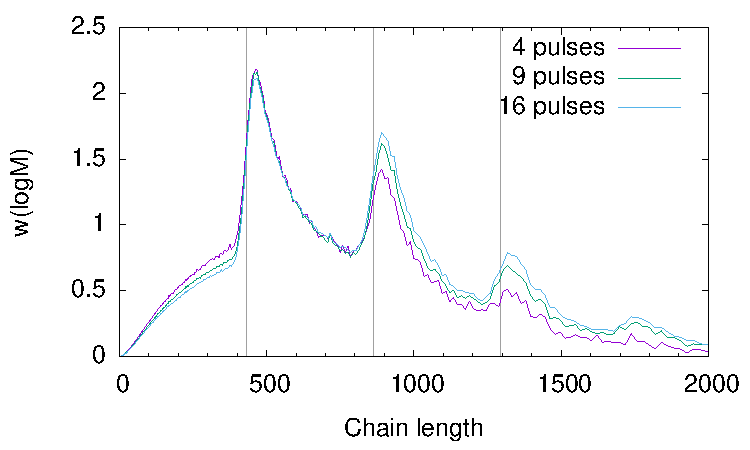
\includegraphics[width=0.77\textwidth]{plp_example3.pdf}
\caption{Results of calculations by mcPolymer with PLP plugin.}
\end{figure}

\begin{figure}[h]
\centering
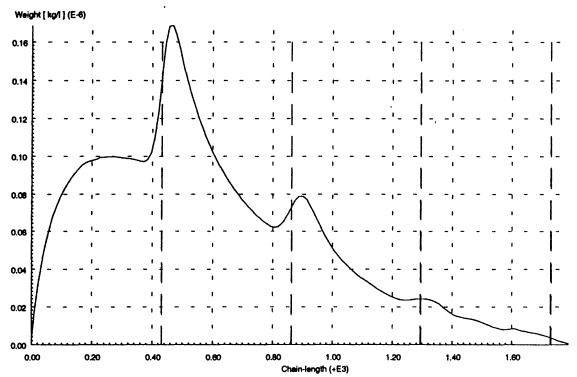
\includegraphics[width=0.8\textwidth]{Wulkow1996_PLP.png}
\caption{Results of calculations by PREDICI published in the paper.}
\end{figure}
\end{document}
